\documentclass[12pt, letter]{article}

% Load packages
\usepackage[style = authoryear, autocite=inline, doi=false,isbn=false,url=false]{biblatex}
\usepackage[margin = 1 in]{geometry}
\usepackage[colorlinks, citecolor = red]{hyperref}
\usepackage{amsmath, amssymb} %essential
\usepackage[long, nodayofweek]{datetime}
\usepackage[]{booktabs}
\usepackage{graphicx}
\usepackage{setspace}
\usepackage{todonotes}
\usepackage[font=small,labelfont=bf]{caption}

% Define symbols
\DeclareRobustCommand{\bbone}{\text{\usefont{U}{bbold}{m}{n}1}}
\DeclareMathOperator{\EX}{\mathbb{E}} % expected value
\DeclareMathOperator{\V}{\mathbb{V}}
\DeclareMathOperator{\Prob}{\mathbb{P}}
\newcommand*{\trans}{^{\mathsf{T}}} %matrix transpose


\begin{document}

% Define Header
\author{Andrew C. Eggers\thanks{Nuffield College and Department of Politics and International Relations, University of Oxford, United Kingdom. \texttt{aeggers@nuffield.ox.ac.uk}}
\and
Tobias Nowacki\thanks{Department of Political Science, Stanford University, CA, United States. \texttt{tnowacki@stanford.edu}}}
\date{\today}
\title{Comparing strategic voting incentives in plurality and instant-runoff elections}

\maketitle

\onehalfspacing % set line space

\setcounter{section}{4}

\section{Data and Methods}

To assess strategic incentives under Plurality and IRV empirically, we rely on data from the  Comparative Study of Electoral Systems (CSES) for a realistic set of preferences and beliefs. The dataset covers 160 surveys from xx different countries, administered shortly before or after an election.\footnote{Two additional cases in the survey, Belarus (20xx) and Lithuania (20xx), are dropped because no respondent specified full preferences over more than two parties.} We focus on the three largest parties (evaluated how?) and label them $A, B, C$ in descending size, respectively. (Some more summary of the data set?)

We construct the utilities over candidates and beliefs over the electoral outcome directly from the CSES data. For (ordinal) utilities, we take CSES respondents' party like/dislike scores (on a scale from 0 to 10) for parties $A, B, C$. This also implies their preferences over the three parties and determines their voter type (e.g., $abc$). For beliefs about electoral outcomes, we proceed as if respondents were presented with full information about everyone else's ordinal utilities. A "Level-1" voter would then believe everyone else to vote sincerely, such that the expected electoral outcome is a vector of ballot shares, $\bf v_j$.\footnote{I am not sure if we can think of this iterative process as just giving voters successive polls, or whether they need to have specific knowledge about others' utilities (probably not).} A "Level-2" voter would believe that everyone else in the sample is a "Level-1" strategic voter, i.e. votes strategically in expectation of a result with sincere voting. The respondent's belief about the probability distribution of electoral outcomes is then given by

\begin{equation}
	f({\bf v}, s) = \text{Dir}(s \times {\bf v})
\end{equation}

where $s$ is a precision parameter (see above). Alternatively, we can think of a Level-2 voter as someone who has just been given a poll of everyone else voting ...(A better way to approach this is probably to start with sincere preferences and then work my way up...)

\subsection{CSES summary statistics}

Brief summary of the CSES dataset (countries, cases, three party dominance)

\emph{Also mentioned in earlier part of Andy's draft -- decide where this belongs}

\subsection{Weights}

Our objective is to characterise the general distribution of strategic incentives under Plurality and IRV under realistic distributions of voters. However, the sample of cases in the CSES dataset is not representative. Some countries have more elections surveyed than others, and there is large variance in countries' electorate. To account for these differences, we use two sets of weights:

\begin{itemize}
	\item when calculating individual-level quantities and aggregating at the level of CSES cases, we use the CSES-provided survey weights for each individual observation.
	\item when calculating aggregate-level quantities and summarising across CSES cases, we use the following weight for each case:
	\begin{equation}
		w_j \equiv 
	\end{equation}
\end{itemize}

\subsection{Iterative Process}

Having described our approach to constructing preferences and beliefs, next we apply the method provided in Section 2 to calculate strategic incentives and voter's optimal ballot if maximising expected utility under either electoral system. In the first instance, we assume that our voters are Level-1 strategic; that is, they expect everyone else to vote sincerely (or have been given a poll where everyone else declares their sincere vote). Let $v_0$ denote the vector of ballot shares if everyone voted sincerely, and $v_1(v_0)$ if everyone voted strategically while having a belief with an expected outcome at $v_0$. 

Of course, when constructing respondents' utilities from like-dislike scores, we cannot know if they would report the same quantities had they been accustomed to a different electoral system (e.g., what if the UK had IRV, rather than plurality?). More generally, if I anticipate others voting strategically, too, I will update my expectations accordingly, and my optimal strategic vote may change as a result. This, in turn, will affect everyone else's optimal choice, and so forth. For that reason, we apply the above method iteratively, until the ballot shares converge onto a fixed-point equilibrium (i.e., where, after updating their expectation about others' strategic votes, no-one changes their vote anymore). [Interpreting the 'learning path'].

\subsection{Quantities of Interest.}
\label{quants}

The iterative algorithm described above yields a large dataset of every respondent's strategic incentive and their optimal ballot for each iteration under either electoral system (all conditional on $s$).

For our analysis, we calculate and present the following quantities of interest in our results section. Each of these quantities is a weighted mean computed for each case within the CSES, conditional on iteration, system, and belief precision. (Express in formal language w/ conditionality).

\textbf{Convergence of strategic voting.} We are interested in what `path' the iterative process described above takes. Specifically, we measure the distance between the iterated result (i.e., the vector of ballot shares) and the original ballot share vector (if everyone voted sincerely). Formally, for iteration $k$, the Euclidian distance is:

\begin{equation}
	d \equiv \sqrt{({\bf v}_k - {\bf v}_0)\trans ({\bf v}_k - {\bf v}_0)}
\end{equation}

\textbf{Prevalence of strategic incentives}. We measure the proportion of voters who have a positive strategic incentive, that is, $\tau_i > 0$ in each setting. Formally, the measure is:

\begin{equation}
	\text{Prevalence} \equiv \Prob(\tau > 0) = \frac{\sum^N_{i = 1} I(\tau_i > 0)}{N}
\end{equation}

\textbf{Magnitude of strategic incentives}. We measure the overall magnitude of these strategic incentives. This is the average of $\tau$ conditional on being greater than $0$.

\begin{equation}
	\text{Magnitude} \equiv \EX[\tau | \tau > 0] = \frac{\sum^N_{i = 1} I(\tau_i > 0) \times \tau_i}{\sum^N_{i = 1} I(\tau_i > 0)}
\end{equation}

\textbf{Expected benefit of strategic incentives}. We measure the expected benefit by asking: on average (across all respondents), what is the expected benefit of strategic voting?

\begin{equation}
	\text{Expected Benefit} \equiv \text{Prevalence} \times \text{Magnitude} = ...
\end{equation}

\textbf{Likelihood of pivotal events}. We measure the likelihood of pivotal events by taking the relevant pivotal probabilities from Section XX (see above). Note that these are conditional on the type of ballot cast and the type of voter -- so for an $abc$ voter, the probability of being pivotal with a $bac$ ballot will be different than that of a $cba$ voter being pivotal with a $bca$ ballot.

(\emph{Does this need formalisation?})

\textbf{Expected cost and benefit of specific ballots}.

Paraphrase Andy's stuff here.



% From each survey in the data set, we take respondents' party like/dislike scores for these parties to approximate voters' ordinal utilities and, by extension, their preferences over the parties.

% Let $\bf \tilde{v}$ be the vector of ballot proportions if everyone in the CSES survey voted sincerely according to their preferences. If voter $i$ believes that everyone else is voting sincerely (in other words, everyone else is Level-0 strategic), then we model the $i$'s belief about the next election as $\text{Dir}(s \times \bf \tilde{v})$, where $s$ is a parameter capturing the precision of $i$'s beliefs. Given this set-up of beliefs and preferences, we calculate the strategic incentives under either electoral system, and iterate this procedure as laid out in Section 3.

% The remainder of this section describes brief summary statistics of the CSES data.


% \subsection{Summary statistics}

% \begin{figure}[!htb]
% 	\centering
% 	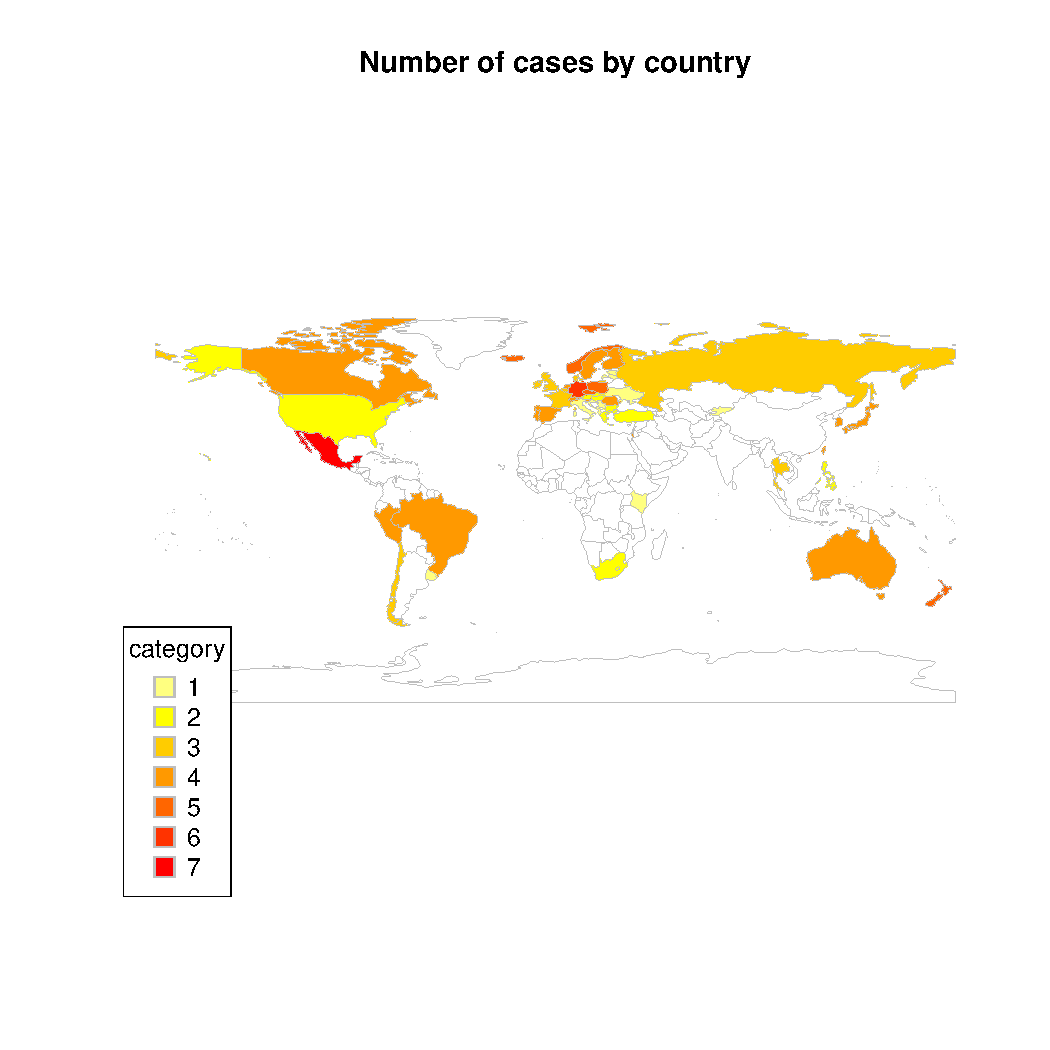
\includegraphics[width = .5 \textwidth]{../output/figures/case_map.pdf}
% 	\caption{Cases in CSES data, by country}
% 	\label{fig:case_map}
% \end{figure}

% The mean number of respondents in the CSES surveys is 1384 (with a standard deviation of 539). The 160 different surveys come from xx different countries, between 1996 and 2016. Figure~\ref{fig:map} maps the number of surveys in each country. (Do we need to say any more? Perhaps something about mean / sd of preference intensity and $\tau$?)

% \subsection{Weighting}

% In some CSES cases, respondents are assigned a non-uniform weight. When computing case-level statistics (e.g., prevalence of strategic incentives in case $j$), we weigh each observation by its original weight. When aggregating up even further, and presenting aggregate statistics (averaged over all cases), we also assign case-level weights to adjust for countries' voting age population and the overrepresenation of some countries.\footnote{Recall that our initial objective is to compare the \textit{overall} distribution of strategic voting incentives under Plurality and IRV. Without weights, we would run the risk of having our findings distorted by a small countryoutlier that counts for as much as a large state (e.g., Denmark and the United States); alternatively, we also do not want a result that is particular to one country to be over-represented purely because there are multiple surveys from that country.}

% These case-level weights are constructed as follows:

% \begin{equation}
% 	w_j \equiv
% \end{equation}

% \subsection{Distribution of preferences} 

% How different are the CSES cases from one another? Aside from the intensity of preferences, we can describe each case with the vector $\bf \tilde{v}$, where the three-item vector $(v_1 + v_2, v_3 + v_4, v_5 + v_6)$ describes the distribution of first preferences, and the three-item vector $(m_{AB} = \frac{v_1}{v_1 + v_2}, m_{BA} = \frac{v_3}{v_3 + v_4}, m_{CB} = \frac{v_6}{v_5 + v_6})$ describes the distribution of second preferences. 

% To link these two distributions together and classify cases more completely, we offer the following approach. Without loss of generality, let the candidate (party) $X$ whose first-preference voters have the most equally split second preferences, and the other two parties $Y$ and $Z$. If both $m_{YZ}$, $m_{ZY} > 0.6$, then classify this case as \emph{single-peaked} and denote it $X+$.\footnote{$X$ is the attractor: both remaining parties have a majority of their second preferences tilted towards $X$.} Conversely, if both $m_{YZ}, m{ZY} < 0.4$, then classify this case as \emph{divided majority} and denote it $X-$.\footnote{Here, $X$ is the repeller: both remaining parties have a majority of their second preferences tilted towards each other and away from $X$.} If $m_{YZ}, m_{ZY} \in [0.4, 0.6]$, then classify this case as \emph{neutral} and denote it $N(X)$. If neither of these conditions hold (because of unusual second preferences), classify it as \emph{other} and denote it $O$. This completes a mutually exclusive and exhaustive set of classes determined by $\bf \tilde{v}$.

% \begin{table}[tb]
% 	\caption{Distribution of preference profiles in CSES data}
% 	\label{tab:csesprefs}
% 	\centering

% 	\begin{tabular}{lccc}
% 	\hline

% 	\toprule
% 	\textbf{} & \textbf{A} & \textbf{B} & \textbf{C} \\
% 	\cmidrule{2-4}
% 	Single-peaked (+) & 18 & 23 & 9  \\
% 	Divided majority (-) & 28 & 20 & 20  \\
% 	Neutral () & 5 & 7 & 3  \\
% 	Other () & & 27 &  \\
% 	\bottomrule
% 	\end{tabular}
% \end{table}

% Table~\ref{tab:csesprefs} summarises the distribution of preference classes across the CSES cases. A plurality of cases belong to the divided majority classes; however, there is also a large number of single-peaked cases, whereas neutral and others tend to be rarer. (Figure~\ref{fig:cses_fp} plots the distribution of first preferences conditional on the classes.)

% \begin{figure}[!htb]
% 	\centering
% 	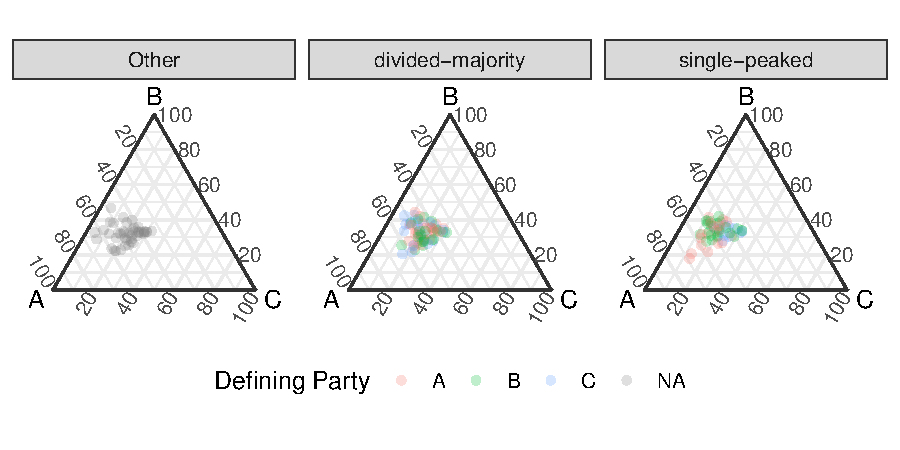
\includegraphics[width = 0.6 \textwidth]{../output/figures/cses_fp.pdf}
% 	\caption{Distribution of first preferences in CSES cases, by class}
% 	\label{fig:cses_fp}
% \end{figure}

\section{Results}

We now proceed to present and discuss our results. For each quantity of interest, we present the average \emph{within} each CSES case (weighted by the respective survey weights) as a thin line across all iterations. We also compute a weighted average \emph{across} all CSES cases for every iteration, which we plot with a thicker line.\footnote{We can interpret this as a `worldwide' average, if you will...}

\subsection{Convergence}

\textit{Main point: show that our cases converge on strategic voting equilibria; in the case of Plurality, two-party ones. Show that these fixed points are further away from original ballot shares under Plurality than under IRV.}

When running our iterative procedure described in detail in Section 2.X.Y, the distribution of ballot shares quickly converges towards a fixed point in the vast majority of CSES cases under both Plurality and IRV. We assume that a fixed proportion $\lambda = 0.05$ of all voters vote strategically in each iteration. The average Euclidean distance going from the 59th to the 60th iteration is below 0.0014 for Plurality, and below 0.006 for IRV.\footnote{These averages are unweighted -- need to recompile in the future.} Put differently, we can obtain a voting equilibrium, where voters anticipate others' vote choices, and react accordingly, within about 60 iterations from the sincere voting profile.

\begin{figure}[!tbh]
	\centering
	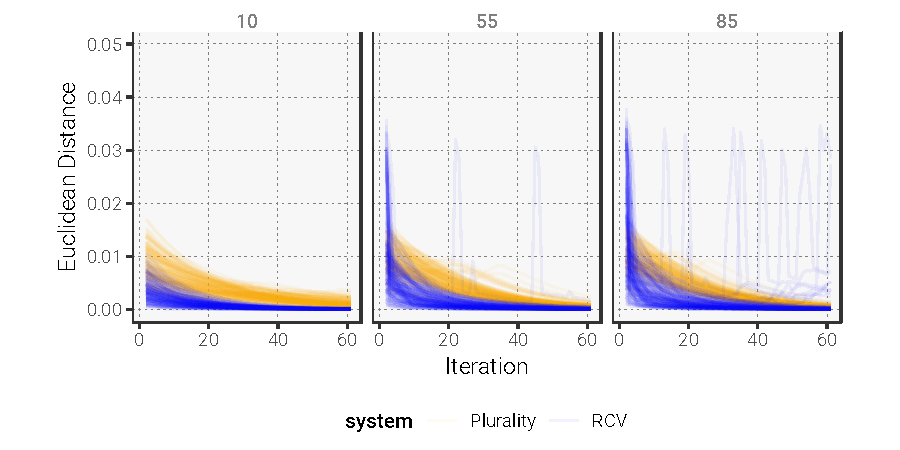
\includegraphics[width = \textwidth]{../output/figures/euclidean}
	\caption{Euclidean distance between ballot share vectors from one iteration to another.}
	\label{fig:convergence}
\end{figure}

Figure~\ref{fig:convergence} plots the Euclidean distance between the ballot shares from one iteration to the next for every case and iteration under both Plurality and IRV. In expectation, convergence towards the fixed point occurs faster under IRV than it does under Plurality. As we discussed earlier, strategic incentives under Plurality are characterised by complementarity; this means that with every additional iteration, the incentive for supporters of the third party increases, until all of them have deserted the trailing candidate and the ballot shares are in a Duvergian (two-party) equilibrium.\footnote{We could visualise this by plotting the share of third-party votes when $k = 60$.} In contrast, the substitutability of strategic voting incentives under RCV allows them to reach a fixed point much sooner: as soon as some $ABC$ voters switch to a strategic ($bac$ or $cab$) ballot, the incentive for myself to do equally lessens. Note however, that, for more precise beliefs ($s \in {55, 85}$), the shift away from the sincere ballot profile in the first few iterations is much bigger than under Plurality; quicker convergence does not necessarily mean that the fixed point is closer to the original ballot share vector. This is also related to the substitution / complementary difference: under Plurality, third-party supporters have an incentive to defect towards the top-two that only increases the more other third-party supporters do so. Consequently, the equilibria under Plurality will be such that all third-party supporters will have deserted their first choice and we end up further away from the original distribution of sincere ballots.\footnote{This foreshadows a later result: with sufficiently high precision, the prevalence of strategic voting incentives under IRV will be higher in the first few incentives.}

In sum, when applying our iterative strategic voting procedure to all CSES cases, the ballot shares converge more quickly to a fixed point under IRV than under Plurality. Under IRV, these fixed points can occur anywhere in the ballot share space, whereas under Plurality, voters ultimately settle on a two-party Duvergian equilibrium. This is also illustrated by Figure~\ref{fig:convergence_paths}, which maps the ballot share vectors before the first and the 60th iteration for $s = 85$.

\emph{(Figure about distance from sincere profile? -- shows nicely that Plurality fixed points are further away from initial ballot shares.)
}
\begin{figure}[]
	\centering
	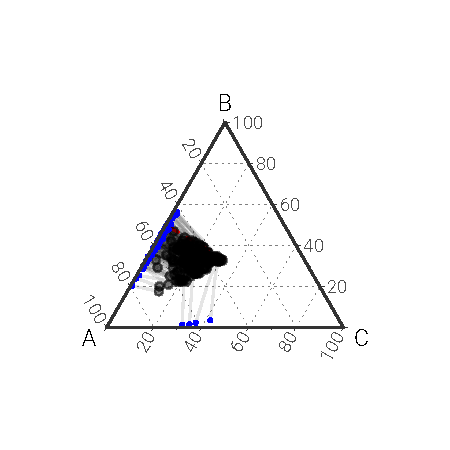
\includegraphics[width = .49\textwidth]{../output/figures/tatonnement_plur}
	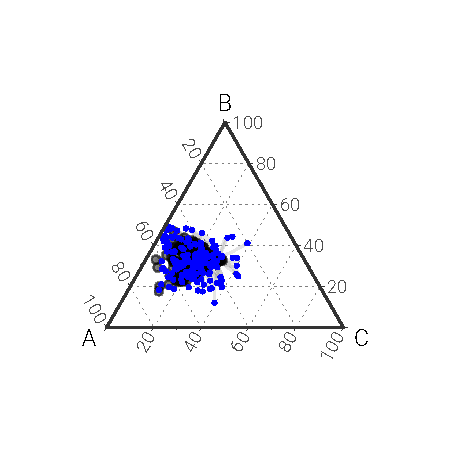
\includegraphics[width = .49\textwidth]{../output/figures/tatonnement_rcv}
	\caption{Evolution of ballot share vectors for all CSES cases over iterations, for both Plurality (left) and IRV (right), when $s = 85$. Grey dots indicate the initial ballot share vector before the first iteration; blue dots the ballot share vector after the 60th iteration.}
	\label{fig:convergence_paths}
\end{figure}

\subsection{Distribution of Strategic Incentives}

% \textit{Main takeaway: discuss expected benefit, magnitude, and prevalence. Show that strategic incentives are, generally speaking, higher under plurality than under IRV. With better information, strategic incentives under IRV become more prevalent, but the benefit of acting on them does not really increase. --> complements and substitudes...}

\emph{two things to add: (a) Across all three quantities, plurality increases with higher precision; (b) discuss magnitude?}

In this section, we characterise the distribution of strategic incentives along the iterative path. We focus on the prevalence, magnitude and expected benefit of strategic voting under either electoral system. Overall, we find that (a) strategic voting incentives are smaller under IRV than they are under Plurality; (b) as precision of beliefs increases, the prevalence of strategic voting incentives increases under IRV as long as voters believe that the vast majority are voting sincerely (lower number of iterations); it does not change much when voters anticipate widespread levels of strategic voting (higher number of iterations); (c)as the anticipation of other voters' strategicness increases, incentives decrease under IRV but increase under Plurality.

We present these results in the form of Figure~\ref{fig:main_stats}, where we plot the weighted average of each quantity within every CSES case conditional on the level of precision (learning path) as a thin line across all iterations. The thicker lines represent the weighted averages aggregated across all CSES cases and are our main point of reference.

\begin{figure}[]
	\centering
	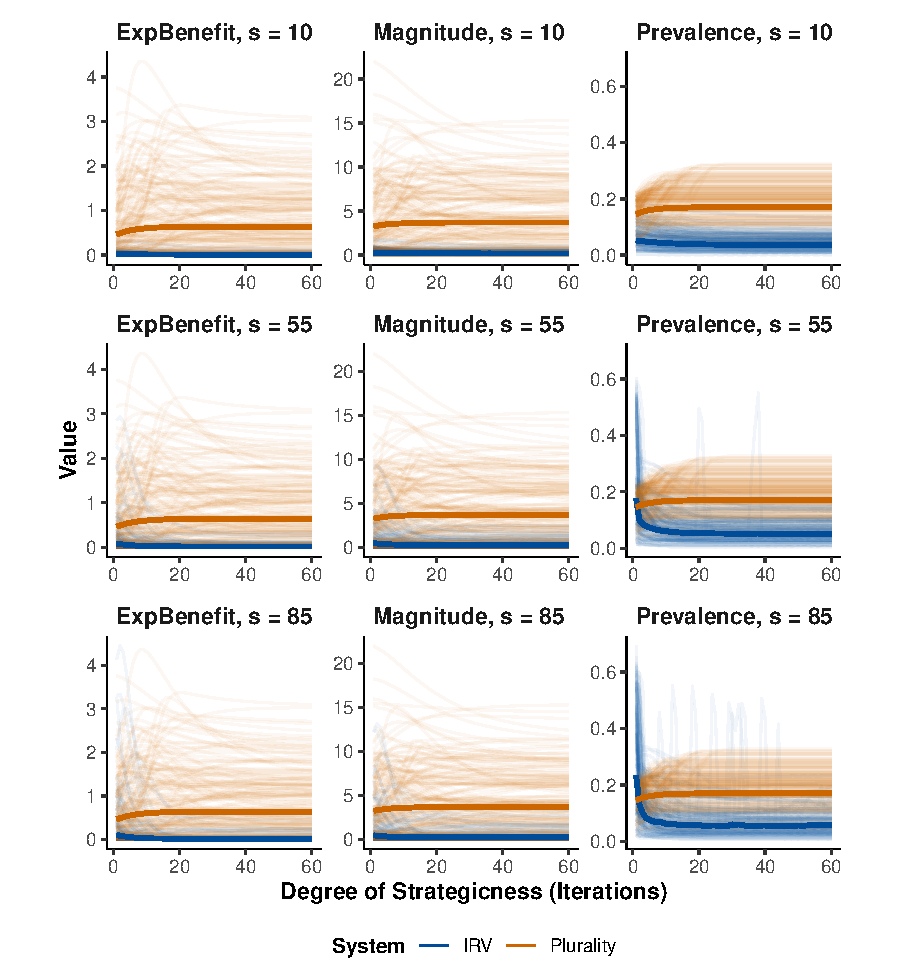
\includegraphics[width = \textwidth]{../output/figures/iterated_complete}
	\caption{Main statistics}
	\label{fig:main_stats}
\end{figure}

First, we note that the average expected benefit of strategic voting is unconditionally higher under Plurality than under IRV. In line with our previous discussion, strategic voting under Plurality is more straightforward and primarily affects those whose first preference is the likely third-ranked candidate. These voters have a straightforward pivotal event (first/second tie) which, by construction, is much more likely than any other; thus, they face little drawback from voting strategically. Under IRV, on the other hand, voters need to be much more careful as the risk of ending up in a situation where the strategic vote backfires is much greater. This confirms the `folk conjecture' that strategic voting incentives under IRV are less widely distributed.

Looking at the prevalence of strategic incentives underlines this intuition: For the most part, incentives are more common in Plurality. However, when the voter anticipates everyone else to vote sincerely (that is, we are at the first iteration) and precision of beliefs is high, the prevalence of strategic voting under IRV is actually quite high (a fifth of the voting population), and slightly higher than that of Plurality. These are the conditions under which a `backfiring' of the strategic vote is least likely. Meanwhile, as we drop to low precision, that incentive becomes less common: with more uncertainty about where the result is going to end up, the risk of casting a `backfiring' strategic ballot becomes greater. For Plurality, the prevalence of strategic voting does not change much across iterations under high precision: with precise beliefs, voters are more certain that their preferred candidate will come last from the onset;\footnote{Unless the second and third are expected to finish very close to one another, of course.} thus already a large proportion of them will desert $C$ from the onset and will continue doing so as more voters become strategic. With more uncertain beliefs, the initial prevalence of strategic incentives under Plurality is lower (as the probability of $C$ tying with either competitor for first place is higher) and increases as strategicness increases and more voters desert $C$ over the course of the iterations.

Finally, we note that as voters become more strategic (that is, we move further along the `learning' path and look at a higher number of iterations), the expected benefit of strategic voting increases under Plurality, but decreases under IRV. This refers back to the difference in the nature of the strategic incentives. Under Plurality, strategic incentives are complements: if I am a supporter of the expected third party $C$, my incentive to desert my preferred choice in favour of the top two increases the more other fellow voters do so, too, as the chance of my preferred $C$ winning decreases even further. Consequently, the incentive to vote strategically increases the more I anticipate others doing so, too. Note that this is most prominent in the case with low precision ($s = 10$). Here, the initial prevalence and magnitude are both lower because with higher uncertainty, there is more of a risk of encountering a first-place tie between $C$ and either $A$ or $B$, in which case a non-sincere ballot for $C$-voters would backfire. As strategicness increases, however, the share of $C$ voters decreases and so does the risk of backfiring.\footnote{Graphically, we are travelling from the centre of the vertex towards the A-B line, as $C$ voters desert their most preferred candidate. It is easy to see how such a movement shifts the distribution away from the $AC$ and $BC$ pivotal lines.}

In contrast, under IRV, strategic incentives are mostly substitutes: if my fellow like-minded voters already vote strategically, then my additional strategic vote may increase the risk of backfiring and accidentally electing the least-preferred option. As a result, the greater the share of anticipated strategic voters, the lower will my own incentives be.\footnote{Since it is hard to judge the degree of strategicness \emph{ex ante}, this poses a fascinating co-ordination problem in real life...}

In sum, the distribution of strategic incentives can be characterised as follows: the average expected benefit of strategic voting is higher in Plurality; with higher precision, the prevalence of strategic incentives improves under either electoral system but more strongly under IRV when voters anticipate everyone else to vote sincerely; finally, as voters' beliefs about others' strategicness increase, the expected benefit increases under Plurality but decreases under IRV.

We continue with the remaining quantities of interest to highlight the points made in this discussion further.

\subsection{Probability of Pivotal Events}

Figure~\ref{fig:pivot} plots the pivotal probabilities for each ballot type as discussed in Subsection~\ref{quants}. Unsurprisingly, the probability is always positive. The average probability of being pivotal with one's strategic vote under Plurality is higher than that of an IRV ballot with one's second preference put first, or that of an IRV ballot with one's third preference put first.

\begin{figure}[!htb]
	\centering
	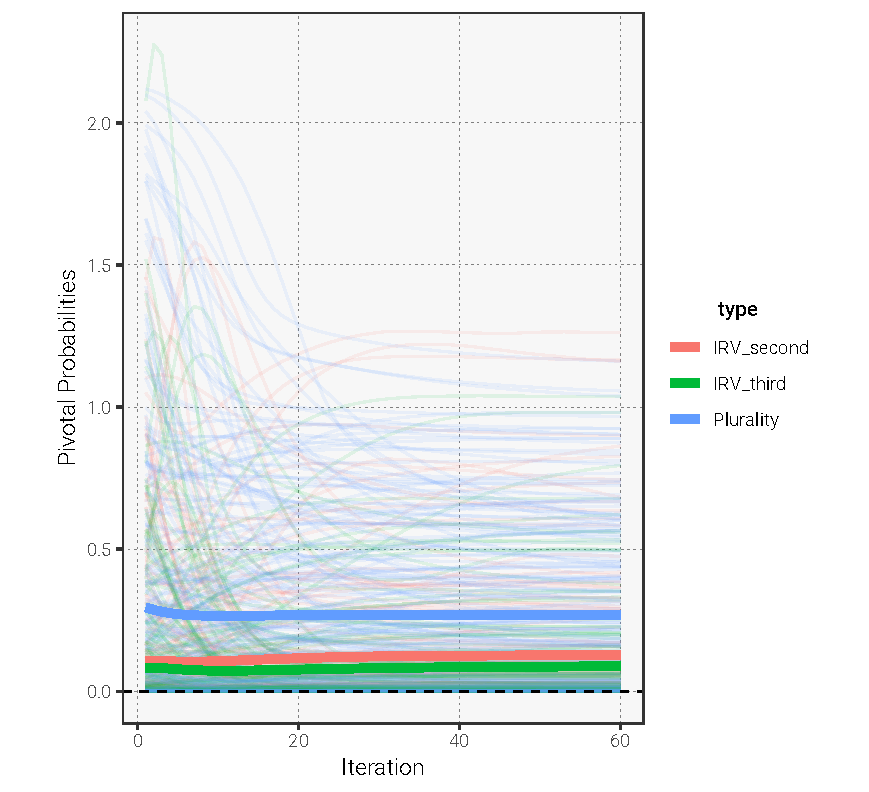
\includegraphics[width = 0.5\textwidth]{../output/figures/conj1}
	\caption{Pivotal probabilities relevant to each strategic vote}
	\label{fig:pivot}
\end{figure}

(\emph{If we keep the conjectures in the text:}) This provides support for conjecture 1.

(\emph{Otherwise:}) Explain / discuss meaning of this along the lines of conjecture 1.

\subsection{Expected Costs and Benefits of Strategic Ballots}

Finally, we report the average correlation between costs and benefits of strategic ballots in Figure~\ref{fig:correlation}.

\begin{figure}[!htb]
	\centering
	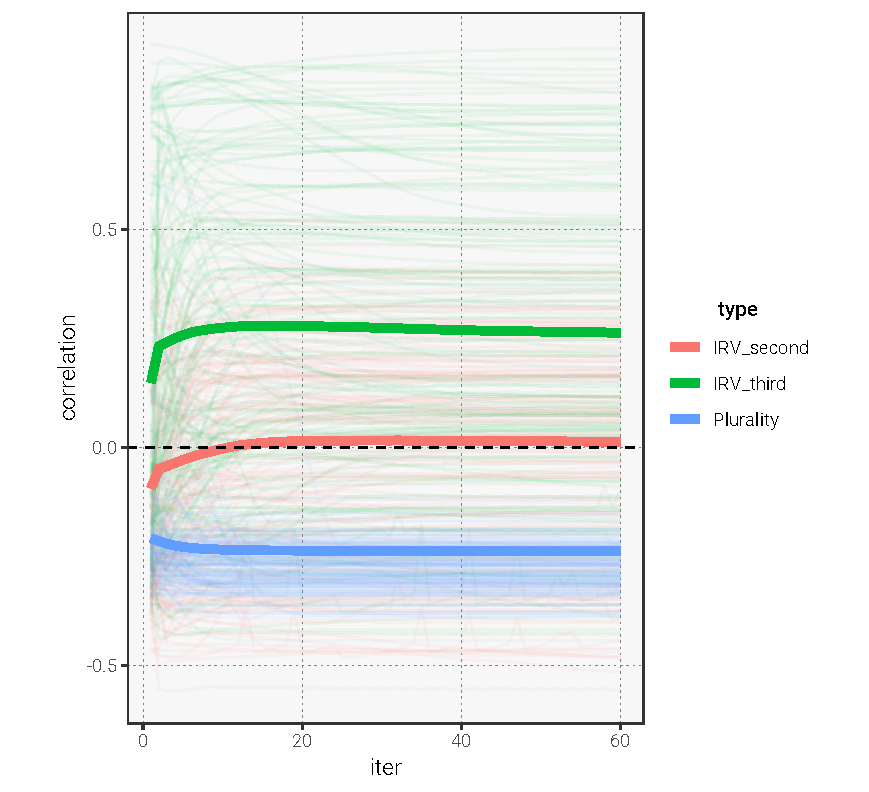
\includegraphics[width = 0.5\textwidth]{../output/figures/conj2}
	\caption{Correlation between costs and benefits of strategic ballots}
	\label{fig:correlation}
\end{figure}

On average, costs and benefits of a strategic ballot in Plurality (voting for one's second preference, rather than sincerely) are negatively correlated. The result supports conjecture 2. This is in line with our previous discussion: the more likely a tie between $A$ and $B$ is (which favours a strategic vote), the less likely will a tie between $C$ and either of the other candidates be (these are the situations where a strategic ballot would be costly). The interpretation under IRV is somewhat less straightforward and depends on whether the strategic ballot puts one's second or third preference first. In the case of an ``IRV-second'' ballot, costs and benefits are, on average, uncorrelated at higher levels of strategicness. (Why?) Finally, in the case of an ``IRV-third'' ballot, costs and benefits are positively correlated. We can interpret this as an increased risk of ``backfiring'': the rewards of putting one's third preference in first position can be high if the right pivotal event occurs, but equally, so are the risks if one ends up with the worst candidate as the winner (and contributed to electing them). Clearly, backfiring carries a greater 

\section{Conclusion}



\end{document}